
\section{f) Implementation and testing}

\textit{There is a collection of benchmark inputs to the classical TSP on the web, see
http://www.iwr.uni-heidelberg.de/groups/comopt/software/TSPLIB95/.
These instances are stored in files following the .tsp file format, see the docu-
mentation on the homepage.
}

\textit{Implement the algorithm you developed in Part d) and run it on certain .tsp
instances, treated as inputs to the optimizing version of LazyTSP. Your software
should at least support those .tsp files where TYPE: TSP and EDGE\_WEIGHT\_TYPE:
EUC\_2D holds, see the file berlin52.tsp for an example. Solutions should be
output along with their costs according to Formula (\(\star\)). Test how the cost of the
solution varies as you increase the parameters k and m.
}

\textit{Instead of developing your software from scratch, you may build upon existing
software packages, provided all legal restrictions are obeyed.
}

The program is implemented in Java. The implementation supports only EUC 2D.
Both algorithms previously described has been implemented.

\subsection{Testing}

The testing provides both the solution and visual output. Testing instructions
are found in the file "README\_TEST".

In the tests performed, it was observed that the depth-search algorithm
had trouble handling input over n - k - m > 10. However, it seemed to scale
somewhat well, being able to handle pla85900.tsp with m = 1 and k = 85892.
In contrast, the greedy algorithm could handle n - m < 20 well, but didn't improve
much from increasing k.

\paragraph{Testing for m + k = c}

Test for eil51.tsp, m+k = 40, depth:

\begin{figure}[h!]
  \caption[Eil51, depth, m+k=40]{m increasing, depth}
  \centering
    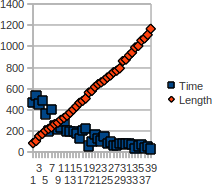
\includegraphics[scale=1.0]{image_1.png}
\end{figure}

Test for eil51.tsp, m+k = 30, greedy:

\begin{figure}[h!]
  \caption[Eil51, greedy, m+k=30]{m increasing, greedy}
  \centering
    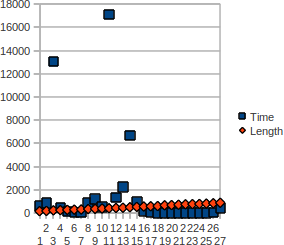
\includegraphics[scale=1.0]{image_2.png}
\end{figure}

The interesting showings from these data sets indicates that the greedy
algorithm seem to have a random running time - most of the time it is decent,
but it has some problems on some input. In fact, it ran out of memory for
m = 29. This seems to show that while the greedy picking of the most promising
path can give a better running time, it gives no guarantees.

Conversely, the depth algorithm clearly benefits from a higher m. It never ran out
of memory. However, it generally cannot handle n - m - k > 10 very well.

In regards to the cost of the solution, it is clear that the solution becomes higher,
the smaller k gets and the higher m gets. This makes intuitively good sense, since
the smaller m is, the more options for picking a more effective solution there are.
Furthermore, the number of nodes to be picked remains constant.

\paragraph{Testing for m = c, k++}

Test for eil51.tsp, m = 20, k = 1..20, greedy:

\begin{figure}[h!]
  \caption[Eil51, greedy]{k increasing, greedy}
  \centering
    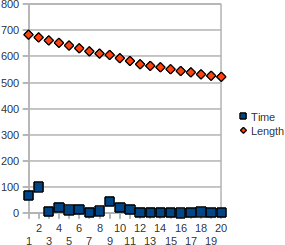
\includegraphics[scale=1.0]{image_3.png}
\end{figure}

As expected, the fewer nodes that has to be included in the cycle,
the smaller the distance becomes.

Test for pla85900.tsp, m = 1, k = 85892..85896, depth:

\begin{tabular}{|l|}
   112368.97433105548 \\
   110476.24692730559 \\
   108638.61430937026 \\
   106856.45151641732 \\
   56400.0 \\
\end{tabular}

Two things are of notice here: First, that the distance decreases as expected when
fewer nodes have to be selected, but that the distance happens not to decrease linearly;
and second, that even though n is very, very large, and m is also very small, the problem
can still be handled when the difference between k and n is very small.
Another thing to notice is that the depth-search algorithm could handle these inputs
without taking much time, while the greedy algorithm happened to fail on lack of memory.

